%preamble
\documentclass[letterpaper]{article}
\synctex=1
\usepackage{graphicx}
\graphicspath{{images/}}

\usepackage{lipsum}
\usepackage{float}

\usepackage{amssymb}
\usepackage{amsmath}

\usepackage{siunitx}
\usepackage{adjustbox}
\usepackage{multirow}
% for merging table cells I think

\usepackage{tabularx}
\renewcommand\tabularxcolumn[1]{m{#1}}% for vertical centering text in X column

% allows for linewrap within cells
\newcolumntype{Y}{>{\centering\arraybackslash}X}

\usepackage{todonotes}
\usepackage{hyperref}

\usepackage{pdfpages} % for attaching the table lol

\usepackage[section]{placeins} % forces figures to appear in the same section

\usepackage[T1]{fontenc}
\usepackage{verbatim}

%for plots
\usepackage{tikz}
\usepackage{pgfplots}
\pgfplotsset{width=8cm,compat=1.15}\usepgfplotslibrary{patchplots}

\usepackage{minted} %code highlighting make sure you have pygmentize installed
\usepackage{xcolor}

\usepackage{csvsimple}

\usepackage[pdf]{graphviz}

\usepackage{pdflscape}
\usepackage{csquotes}
\usepackage{enumitem}
\usepackage{lastpage}

\renewcommand*\contentsname{Table of Contents}

\def\me{Arun Woosaree\\ XXXXXXX}
\usepackage[english]{babel}
\usepackage[utf8]{inputenc}
\usepackage{fancyhdr}
\pagestyle{fancy}
\fancyhf{}
\rhead{\me}
%\lhead{Guides and tutorials}
\cfoot{Page {\thepage} of {\pageref{LastPage}}}

\title{ECE 315 Assignment 1}
\author{\me}

\begin{document}
\maketitle

\section{}
\subsection*{}
The system will enter any of the low power modes below when a \texttt{STOP}
instruction is executed. Depending on the \texttt{WCR[LPMD]} bits, the MCU will
enter either wait, doze, or stop mode.
For each of these modes, power is saved by idling the CPU with no active
cycles, powering down the system, and stopping all internal clocks. The coldfire
core is also disabled in each of the low-power modes. 

A wake-up event will cause the MCU to exit any of these low power modes, and
return to run mode. A wake-up event can be any type or reset, or any valid,
enabled interrupt request. To exit from these low power modes with an interrupt,
the interrupt request's priority should be higher than the value programmed in
\texttt{WCR[LPMD]}, and higher than the value programmed in the interrupt
priority mask (I) field of the core’s status register. Additionally, the
interrupt request should be from a source that is not masked in the interrupt
controller’s interrupt mask register, and it should have been enabled at the
module of the interrupt’s origin.

\subsubsection*{wait} 
Wait mode saves power by stopping the CPU and memory clocks until a wake-up
event is detected. Peripherals can be programmed to continue operating, and can
also generate interrupts which will cause the CPU to exit from wait mode. The
wait mode is entered when the \texttt{STOP} instruction is executed, with the
\texttt{WCR[LPMD]} bits having a value of \texttt{10}.

%A wake-up event will cause the MCF54415 to exit wait mode.
\subsubsection*{doze} 
Doze mode is similar to wait mode, in that it affects the
processor in the same way as in wait mode, however, some peripherals define
individual operational characteristics in doze mode. Peripherals continuing to
run and having the capability of producing interrupts may cause the CPU to exit
the doze mode and return to run mode. Stopped peripherals restart operation on
exit from doze mode, as defined for each peripheral
The doze mode is entered when the \texttt{STOP} instruction is executed with the
\texttt{WCR[LPMD]} bits having a value of \texttt{01}.

\subsubsection*{stop}
Stop mode is also similar to wait and doze mode, in that it affects the
processor the same way. However, all system clocks are stopped, and peripherals
cease operation.
The stop mode is entered when the \texttt{STOP} instruction is executed with the
\texttt{WCR[LPMD]} bits having a value of \texttt{11}.

%The SRAM, Power Management, Chip Configuration Module, System Control Module,
%GPIO, Edge Port, eDMA Controller, FlexBus Module, DDR Controller, USB OTG, USB
%Host, SSI, Programmable Interrupt Timers, DMA Timers, 

\section{}

The FIFO buffer in the FEC helps with handling short term burstiness of the data
that is both recieved by the FEC and transmitted from the FEC from the CPU. If
the CPU cannot keep up for a moment with sending bits or receiving bits fast
enough, the buffer ensures that data is available to be processed when the CPU
is ready without having to abandon or truncate packets. 


The DMA allows for data to be transferred more efficiently between the system's
memory, and the FIFO buffer in the FEC. The DMA controller allows for the
movement of blocks to take up less CPU cycles, since the direct memory access is
done in place of a bunch of CPU move instructions.

If the system designer is expecting more bits to be sent than recieved, they may
choose to partition the FIFO buffer such that more space is allocated for
sending bits than receiving. Similarly, if more bits are expected to be received
than sent, then the FIFO buffer may be allocated such that the buffer for
receiving is larger. 

This decision would be implemented by loading the value \todo{i dunno}


into an FEC register.

\section{}
\subsection*{Advantages}
\begin{itemize}
  \item All ethernet frames will fit in the buffer
\end{itemize}

\subsection*{When would it be more appropriate to choose a single threaded
  bare-metal architecture}

\begin{itemize}
  \item THe FEC would accept frames that are larger than the ethernet standard
    and are potentially garbage
\end{itemize}

A pointer can be created in the following ways:
\begin{enumerate}
  \item You can ask the OS to allocate a region of
    memory using \texttt{malloc()}, \texttt{calloc()}, or \texttt{realloc()},
    and give you a pointer to that region of memory. It is up to the programmer
    to check if NULL was returned and deal with error handling.
  \item The \texttt{\&} operator is used to obtain a pointer to an existing
    piece of data
  \item math is done on an existing pointer, and the result is stored as a new
    pointer. (e.g. \texttt{char* new\_ptr = other\_ptr + 8})
  \item A pointer can be declared but uninitialized. A so-called wild pointer
    can point to anywhere in memory and therefore should not be used. A pointer
    should be initialized with a value before use.
\end{enumerate}

Throughout a pointer's life, it can be modified and overwritten. An example of a
pointer being modified would be a typed pointer being incremented or decremented
before or after they are used. (e.g. \texttt{*(ptr++)}.  Void pointers, which
can be used to point to anything can be casted to a different type before being
modified (e.g. \texttt{ptr = (char* ptr)}) as well. Also, a pointer can be
overwritten by simply assigning another pointer value to the existing pointer.

When the value a pointer to no longer needs to be used, a responsible C
programmer will call \texttt{free()} to recycle the memory.
Once the block of memory that a pointer points to is freed using the
\texttt{free()} function, the pointer can be safely discarded. Actually, the
pointer should no longer be used, because the pointer now points to a region of
memory that has been recycled. This is called a dangling pointer. Failure to
call \texttt{free()} after the object is no longer required results in what is
known as a memory leak.


\section{}
There are two different systems of priorities because tasks and hardware
interrupts are meant to behave very differently from each other. Hardware
interrupts usually are meant to interrupt tasks that are currently running, so
that the system can react in real-time to external events, while tasks generally
have lower priority. For example, waking up the system from a low-power state
happens with a hardware interrupt, and stops the idle task from running. This is
an example of the two different systems interacting. These
two systems can also interact with each other when a task requires a hardware
interrupt to continue execution. For example, waiting on a hardware timer, or an
I/O request.

\section{}

A ping-pong buffer is a double buffer that can be used to overlap I/O operations
with data processing to speed up a device.  The idea is that the first buffer
holds some old, but complete data which the reader can access, while the other
buffer holds some partial, incomplete but newer data which the writer is writing
to. When the writer is finished, the buffers switch and "ping-pong", so that the
reader is now reading from the second buffer, and the writer is writing to the
first buffer. This process repeats itself.
An illustration from the notes is below:

  \includepdf[pages={17}, width=\textwidth]{../../notes/Ch11_W20_Flow_Control.pdf}

  The advantage of a ping-pong buffer is that the reader and the writer can
  access data stored in their respective buffers in any arbitrary order,
  as opposed to a FIFO buffer for example, which requires that the data is read
  in the same order as it was written in. 

  For example, if an application was doing matrix operations, the elements of a
  matrix could be written column-by-column, while the reader could read the
  matrix row-by-row.

  Another example application where a ping-pong buffer may be useful is in
  streaming video. The data in one buffer can be sent to a graphics card to
  display the video to the user, while at the same time, another buffer is being
  written to by the network card, where the video stream is coming from.

\section{}
If we start at the closed state, we can transition to the listening state if
passive open???

Next, if a syn is recieved, or a syn + ack, we reach the syn recieved state.
From there, if an ack is recieved, we then reach the established state. 

The system would fall behind on its real-time guarantees if the amount of idle
time was reduced below a safe percentage of the CPU' execution time. 

For externally initiated events, too little idle time would mean not enough
excess CPU capacity so that the worst-case bursts of event-handling workloads
would not be able to be handled within the maximum response time variability
specifications. 

For internally initiated events, not enough idle time would mean that the
effects of internal sources of timing variability (e.g., variability in the
execution time of compiled software, cache memory and virtual memory,and DMA
activity) would not be absorbed and therefore not hidden. 
%The timing for internally initiated events should be determined by H/W timers.

You would start to see problems like the system being less responsive, and
longer wait times for tasks to complete due to lower priority tasks not getting
a chance to run as often. (With the idle task being the lowest priority task, if
it does not run often, that means that other lower priority tasks likely also
did not get many chances to run.)


\end{document}
